\section{Expected Outcomes}

CPS market accounted for almost \euro 472 billion in the automotive, industrial, medical, aerospace and defence industries in 2012\footnote{\url{https://ec.europa.eu/digital-single-market/en/news/european-industrial-strategic-roadmap-micro-and-nano-electronic-components-and-systems}}. By improving the development of dependable CPS and supporting the ad-hoc connection of dependable systems during field operation, DEIS holds the opportunity to bring a significant impact on the existing market and be an enabler for future solutions based on dependable CPS. 

For the automotive market, providing means for ensuring dependability of collaboration at runtime will be the enabler to gain market shares in novel market segments. For the railway market, in particular, European rail transport, the harmonisation and supervision of safety certification are essential in a Single European Railway Area and for railway suppliers to deliver cost-efficient and quality products. For the healthcare market, the need for improved science system integration for dependable, autonomous and connected CPS is also imperative.

The expected outcomes based on the objectives mentioned in Section \ref{section4} are:

\begin{enumerate}
	\item Definition of the ODE metamodel and the specification of DDI. 
	\item A semi-automated framework for the generation and evaluation of DDIs.
	\item A framework for the in-the-field dependability assurance in CPS.
	\item Autonomous and connected CPS use cases, which is shown in Figure \ref{fig:impacts}.
\end{enumerate}

\begin{figure}[ht!]
	\centering
	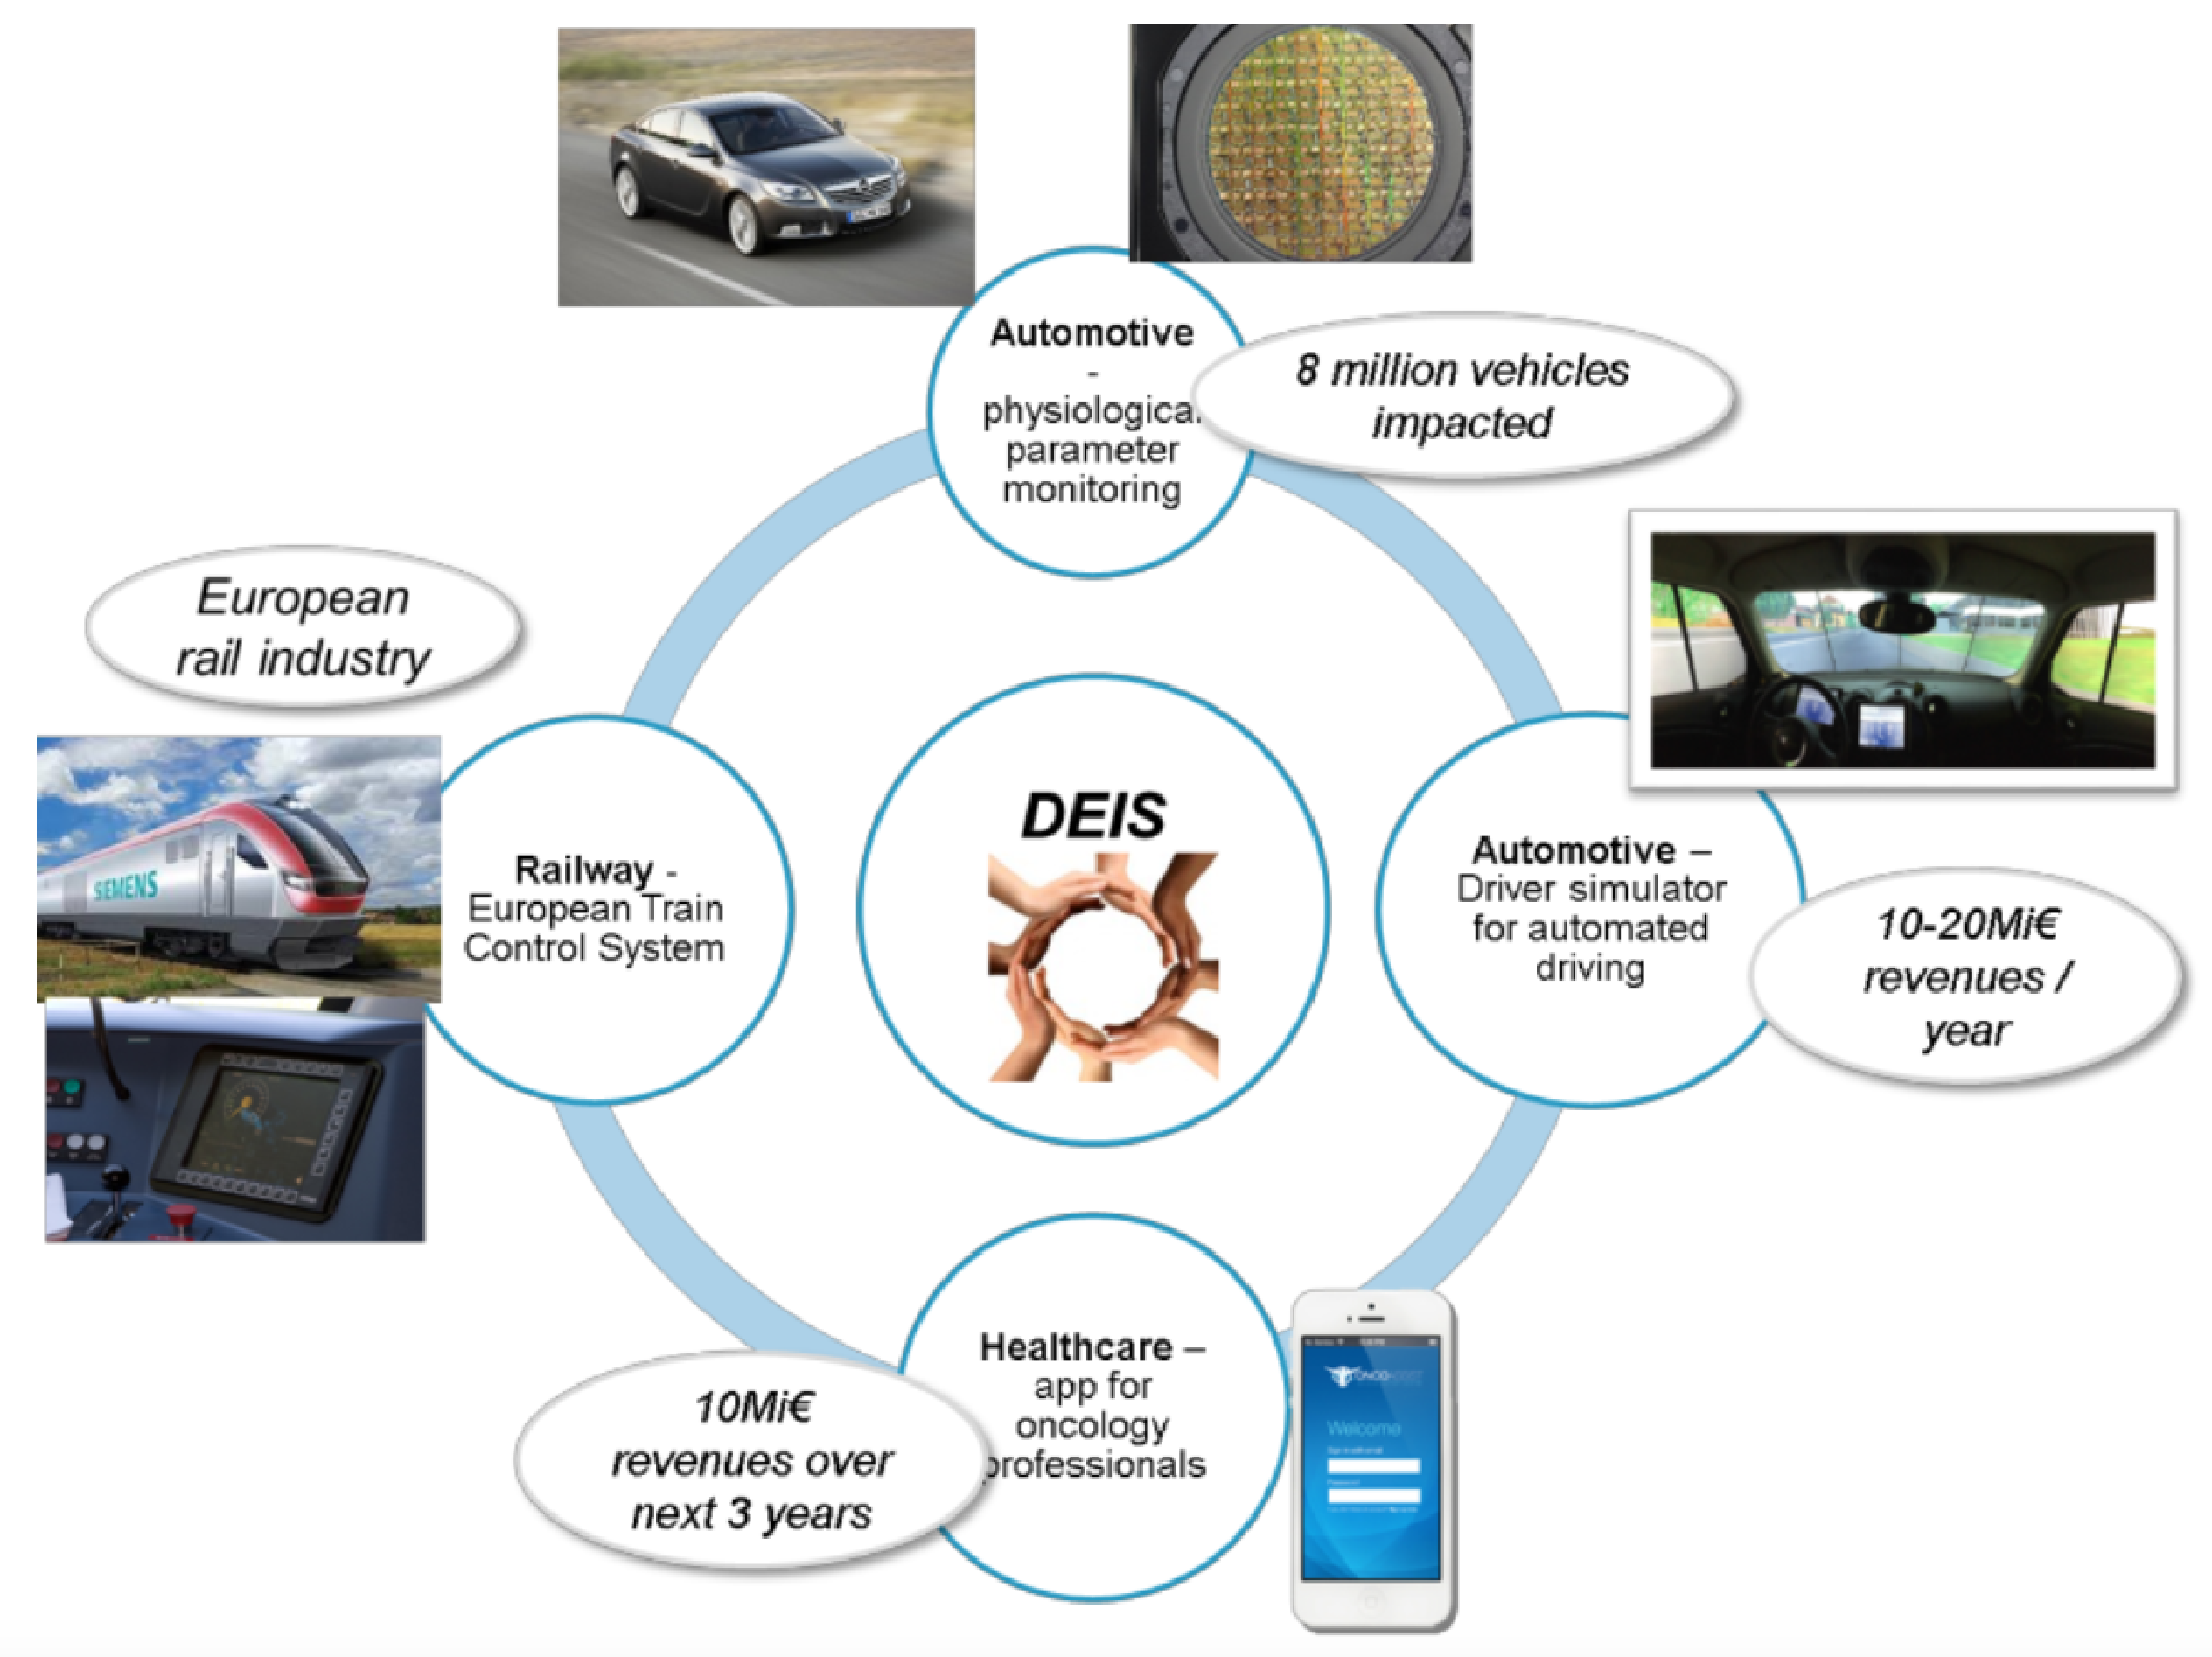
\includegraphics[width=0.87\linewidth]{./fig/usecase_impacts.pdf}
	\caption{Expected impact of the use cases on their respective markets.}
	\label{fig:impacts}
\end{figure}